\subsection{Pi}

Her beskrives intern kommunikation for controlleren PI i systemet. 

\begin{figure}[h]
\centering
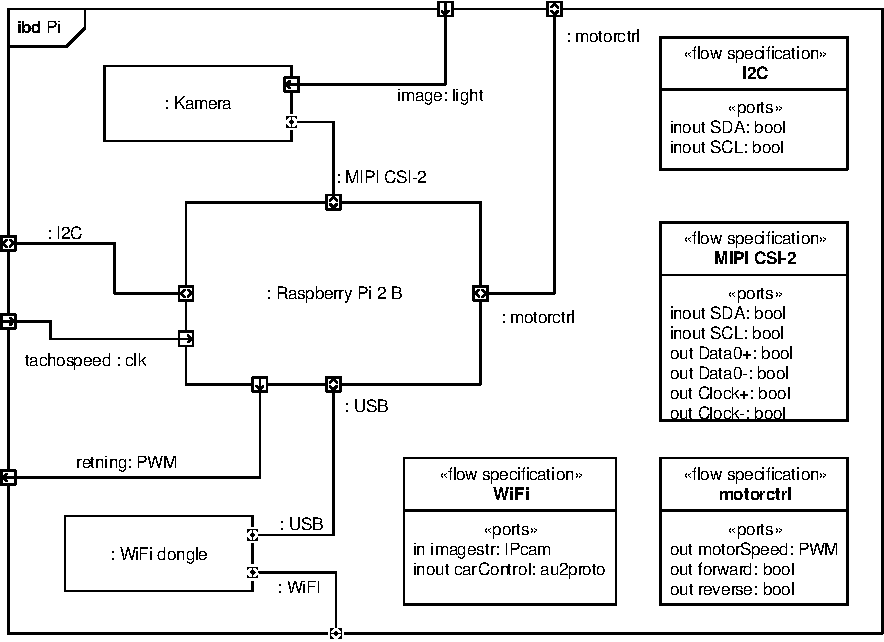
\includegraphics[scale=1]{../fig/diagrammer/bil/ibd_pi.pdf}
\caption{IBD for blokken PI}
\label{fig:ibd_pi}
\end{figure}


\subsubsection{Signalbeskrivelse for Pi}

\begin{table}[h]
	\centering
	\begin{tabularx}{\textwidth}{|l|X|X|X|} \hline
	\textbf{Signal (navn: type)} & \textbf{Funktion} & \textbf{Tolerancer} & \textbf{Kommentarer} \\ \hline
SDA: bool
	& I2C dataline til sensorer herunder accelerometer og afstandssensorer  
	& 0-5V$\pm$0.5V 
 	& Logisk signal: 			\newline
		Lav= 0V$\pm$0.5V  	\newline
		Høj= 7.2V$\pm$0.5V
	\\ \hline
	
SCL: bool
	& I2C clockline  til sensorer herunder accelerometer og afstandssensorer
	& 0-5V$\pm$0.5V
	& Logisk signal:			\newline 
		Lav= 0V$\pm$0.5V 	\newline
		Høj= 7.2V$\pm$0.5V
	\\ \hline
	
Image: light
	& Lysindfald til kamerasensor
	& -
	& -
	\\ \hline

motorSpeed: PWM	
	& Et PWM signal der bestemmer motorhastigheden.	
	& Frekvens: 30kHz$\pm$1kHz \newline
	  0-5V$\pm$0.2V	
	& Logisk signal: 			\newline 
		Lav= 0V$\pm$0.2V 	\newline
		Høj= 5V$\pm$0.2V
	\\ \hline
	
forward: bool	
	& Kontrolsignal til H-bro
	& 0-5V$\pm$0.2V
	& Logisk signal:					\newline 
		Lav= 0V$\pm$0.2V  ''idle''		\newline
		Høj= 5V$\pm$0.2V  ''forward''
	\\ \hline
	
reverse: bool	
	& Kontrolsignal til H-bro
	& 0-5V$\pm$0.2V	
	& Logisk signal: 					\newline
		Lav= 0V$\pm$0.2V ''idle''		\newline
		Høj= 5V$\pm$0.2V ''back''
	\\ \hline
	
:USB 	
	& Serielforbindelse mellem Wi-fi dongle og Pi	
	& VBUS = 5V$\pm$0.2V 				\newline 
	  D$-$ = 5V$\pm$0.2V					\newline
	  D$+$ = 5V$\pm$0.2V					\newline
	  GND = 0V							\newline	  
	  & VBUS for Low-power port: 		\newline
		Diff  ''1''						\newline
		(D$+$)-(D$-$) > 200 mV				\newline
		og D$+$>VIH (min)					\newline

		Diff ''0''						\newline
		(D$-$)-(D$+$) > 200 mV				\newline
		og D$-$>VIH (min)					\newline
	\\ \hline	
	
imagestr: IPcam
	& Karsten... Dette er dit job %TODO Karsten 
	& - 
	& -	
	\\ \hline

carControl: au2proto
	& Få fingeren ud Karsten. %TODO Karsten
	& -
	& -
	\\ \hline
	
: MIPI CSI-2
	& Camera serial interface
	& -
	& Se reference: \cite{lib:MIPICSI-2}
	\\ \hline
	\end{tabularx}
\end{table}
